\documentclass[10pt,twocolumn]{article}

\usepackage{times}
\usepackage{fullpage}

\usepackage{booktabs}  % for \midrule
%\usepackage{subfigure}
\usepackage{balance}
\usepackage{graphicx}
\usepackage{xspace}
\usepackage{amsmath}
%\usepackage{pslatex}
%\usepackage{pifont}
%\usepackage{multirow}
%\usepackage{array}
%\usepackage{booktabs}
%\usepackage{cite}
\usepackage{url}
%\usepackage{cancel}
\usepackage{color,colortbl}
%\usepackage{microtype}
%\usepackage{textcomp}% http://ctan.org/pkg/textcomp
\usepackage{tabularx}
\usepackage{framed}
\usepackage[]{algorithm2e}
\SetAlFnt{\small}
\SetAlCapFnt{\small}
\usepackage{algorithmic}

\usepackage{listings}
%\usepackage{scrextend}
%\usepackage{mathtools}
\usepackage{pbox}
\usepackage{subcaption}

\let\labelindent\relax
\usepackage{enumitem}

\usepackage{tikz}
\usetikzlibrary{arrows,automata}
\usetikzlibrary{calc,positioning}
\usepackage{lipsum,adjustbox}

%\usepackage{tikz}
%\usepackage{decorations.pathmorphing}
%\usepackage{assymb}

\usepackage[labelfont=bf]{caption}

%\theoremstyle{plain}
\newtheorem{theorem}{\bf{Theorem}}%[section]
\newtheorem{lemma}[theorem]{\bf{Lemma}}
\newtheorem{corollary}[theorem]{\bf{Corollary}}
\newtheorem{proofl}[theorem]{\bf{Proof}}
\newtheorem{proposition}[theorem]{\bf{Proposition}}

%\theoremstyle{definition}
\newtheorem{definition}{\bf{Definition}}%[section]
\newtheorem{observation}{\bf{Observation}}%[section] 

%\theoremstyle{remark}
\newtheorem{example}{\bf{Example}}
\newtheorem{notation}{\bf{Notation}}
\newtheorem{fact}{\bf{Fact}}

\usepackage{listings}
%%\usepackage{listings-golang}
\usepackage{color}

\definecolor{dkgreen}{rgb}{0,0.6,0}
\definecolor{gray}{rgb}{0.5,0.5,0.5}
\definecolor{mauve}{rgb}{0.58,0,0.82}

\lstset{frame=tb,
  language=Java,
  aboveskip=3mm,
  belowskip=3mm,
  showstringspaces=false,
  columns=flexible,
  basicstyle={\small\ttfamily},
  numbers=none,
  numberstyle=\tiny\color{gray},
  keywordstyle=\color{blue},
  commentstyle=\color{dkgreen},
  stringstyle=\color{mauve},
  breaklines=true,
  breakatwhitespace=true,
  tabsize=3
}

%\usepackage{sectsty}
%\sectionfont{\fontsize{12}{15}\selectfont}

\usepackage{hyperref}

\newcommand\mypara[1]{\vspace{.3em}\noindent\textbf{#1}}
\newcommand{\urlwofont}[1]{\urlstyle{same}\url{#1}}


%%%%%%%%%%%%%%%%%%%%%%%%%%%%%%%%%%%%%%%%
% Useful reviewing/feedback annotations
\usepackage{ifthen}
\usepackage[normalem]{ulem} % for \sout
\usepackage{xcolor}
\usepackage{amssymb}

\newcommand{\ra}{$\rightarrow$}
\newboolean{showedits}
\setboolean{showedits}{true} % toggle to show or hide edits
\ifthenelse{\boolean{showedits}}
{
	\newcommand{\ugh}[1]{\textcolor{red}{\uwave{#1}}} % please rephrase
	\newcommand{\ins}[1]{\textcolor{blue}{\uline{#1}}} % please insert
	\newcommand{\del}[1]{\textcolor{red}{\sout{#1}}} % please delete
	\newcommand{\chg}[2]{\textcolor{red}{\sout{#1}}{\ra}\textcolor{blue}{\uline{#2}}} % please change
}{
	\newcommand{\ugh}[1]{#1} % please rephrase
	\newcommand{\ins}[1]{#1} % please insert
	\newcommand{\del}[1]{} % please delete
	\newcommand{\chg}[2]{#2}
}

\newboolean{showcomments}
\setboolean{showcomments}{true}
%\setboolean{showcomments}{false}
\newcommand{\id}[1]{$-$Id: scgPaper.tex 32478 2010-04-29 09:11:32Z oscar $-$}
\newcommand{\yellowbox}[1]{\fcolorbox{gray}{yellow}{\bfseries\sffamily\scriptsize#1}}
\newcommand{\triangles}[1]{{\sf\small$\blacktriangleright$\textit{#1}$\blacktriangleleft$}}
\ifthenelse{\boolean{showcomments}}
%{\newcommand{\nb}[2]{{\yellowbox{#1}\triangles{#2}}}
{\newcommand{\nbc}[3]{
 {\colorbox{#3}{\bfseries\sffamily\scriptsize\textcolor{white}{#1}}}
 {\textcolor{#3}{\sf\small$\blacktriangleright$\textit{#2}$\blacktriangleleft$}}}
 \newcommand{\version}{\emph{\scriptsize\id}}}
{\newcommand{\nbc}[3]{}
 \renewcommand{\ugh}[1]{#1} % please rephrase
 \renewcommand{\ins}[1]{#1} % please insert
 \renewcommand{\del}[1]{} % please delete
 \renewcommand{\chg}[2]{#2} % please change
 \newcommand{\version}{}}
\newcommand{\nb}[2]{\nbc{#1}{#2}{orange}}

\definecolor{ibcolor}{rgb}{0.4,0.6,0.2}
\newcommand\iv[1]{\nbc{IB}{#1}{ibcolor}}
\usepackage{wasysym}
\newcommand\yesml[1]{\nbc{ML {\textcolor{yellow}\sun}}{#1}{mircolor}}

\definecolor{sgcolor}{rgb}{0.2,0.0,0.5}
\newcommand\sg[1]{\nbc{SG}{#1}{sgcolor}}

\definecolor{samcolor}{rgb}{0.2,0.4,0.2}
\newcommand\sam[1]{\nbc{SC}{#1}{samcolor}}

\definecolor{hccolor}{rgb}{0.21,0.54,0.84}
\newcommand\hc[1]{\nbc{HC}{#1}{hccolor}}

\definecolor{ideacolor}{rgb}{1.0,0,0.5}
\newcommand\idea[1]{\nbc{IDEA}{#1}{ideacolor}}


\definecolor{abstractcolor}{rgb}{0.0,0.5,1.0}
\newcommand\rabstract[1]{\nbc{ABSTRACT}{#1}{abstractcolor}}

\definecolor{introcolor}{rgb}{0.0,1.0,0.5}
\newcommand\rintro[1]{\nbc{INTRO}{#1}{introcolor}}

\definecolor{papercolor}{rgb}{1.0,1.0,0.0}
\newcommand\rpaper[1]{\nbc{PAPER}{#1}{papercolor}}

\definecolor{multicolor}{rgb}{1.0,0,0}
\newcommand\rmulti[1]{\nbc{MULTI}{#1}{multicolor}}

% Todo Command
\definecolor{todocolor}{rgb}{0.9,0.1,0.1}
\newcommand{\todo}[1]{\nbc{TODO}{#1}{todocolor}}


%%%%%%%%%%%%%%%%%%%%%%%%%%%%%%%%%%%%%%%%


\begin{document}

%\title{Inferring likely data invariants of distributed systems}
\title{RDMAttack! or how I learned to stop worrying and authenticate at line rate}

\author{Stew, Shu-Ting, Yibo
\\ University of California San Diego}
\date{}

\maketitle

\section{Abstract}
\label{sec:abstract}

RDMA over converged ethernet (RoCEv2) is a high performance network protocol
for directly accessing the memory of a remote machine by bypassing its CPU.
The protocol's design prioritizes performance above all else, leaving security
properties such as authenticity and confidentiality by the wayside. Security is
largely unnecessary in the intimately coupled compute clusters RoCEv2 was
designed for. RDMA's performance benifits have been widely recognized, and it
has been integrated into a wide set of dataceter applications. Many of these
general purpose applications run on diverse sets of machines (sometimes across
data centers) which has propelled RDMA into high risk environments it was never
designed for.

In this work we consider the design of secure RDMA. As motivation for the redesign,
we hijack RDMA by performing a trivial man in the middle attack. We show that
an unsophisticated attacker in control of a switch's routing table can gain
full control over plaintext RDMA payloads, reading and writing to arbitrary victim addresses.
Securing RDMA requires careful consideration of its performance; practitioners
will not adopt a solution which degrades their high performance applications.
We benchmark common encryption algorithms and demonstrate that commodity CPU's
cannot encrypt at the beefy bandwidth's (100 and 400Gbps) RDMA is designed for.
Our conclusion is that RDMA encryption must be implemented as a NIC offloaded
function to achieve line rate performance.

\section{Introduction}
\label{sec:intro}

RDMA (Remote Direct Memory Access) is a high performance network protocol that offers microseconds latency and hundreds of gigabits throughput,
which can significantly benefit high performance computing as well as data intensive workload. RDMA was initially designed to run over InfiniBand network,
and was mostly used in HPC clusters. Its high performance characteristics comparing with traditional TCP/IP stack lead to the standardization of RoCE,
RDMA over Converged Ethernet, and significantly improved the performance of modern datacenter applications like \texttt{memcached}, \texttt{Spark} and \texttt{Tensorflow}.

Originally designed for HPC environment, RDMA has very little built-in security features. Other than a 32-bit remote key for RDMA read/write requests,
there is no security feature other than standard CRC for detecting link-level bit errors. Previous work like ThrowHammer~\cite{216055} has shown that
it's possible to launch local-only memory attack over RDMA, due to its high message rate capability. In addition, an attacker can also perform a
denial-of-service attack by injecting RDMA request at high speed, or by sending large amount of read requests, which are small themselves, but
generates large amount of data to be sent in responses.

In this paper, we will show that it is possible for an attacker to launch a man-in-the-middle attack. Realisticly, this means that in a datacenter,
a malicious user compromised a switch and thus is able to view and modify traffic going through the switch. We show that without proper protection,
normal application traffic can be hijacked. We describe the proof-of-concept attack and show its feasibility in \autoref{sec:poc.attack}.

This motivates many potential defense mechanisms, two of which are encrypting and authenticating the traffic end-to-end.
We show in \autoref{sec:encrypt} that modern datacenter server CPUs need at least several cores solely
for encrypting/hashing traffic at line rate, which is around $40 - 100$ Gbps for modern NICs.
Our result shows that NIC offloading or accelerator is the preferred way to achieve such RDMA security goals at line rate.


\todo{After migrating the original intro back make sure to talk about denial of service attacks as a potential extension of RDMA attacks. Denial of service happens in a few forms}

\todo{1 Read amplification an attacker who knows the key of a memory region can flood the network by injecting a large number of read requests causing the node responsible for the data to attack the network blindly.}


\todo {2 an opaque attack can also be made by adjusting the offset of the read, a fast attack which only requires the update of the checksum and the read size.}




\section{Background}
\label{sec:background}

\begin{itemize}
    \item{TLS}
    \item{RoCE}
    \item{iWARP}
    \item{Secure RDMA}
\end{itemize}

\begin{itemize}
\item{Security Enhancement in InfiniBand Archetecture}~\cite{Lee:2005:SEI:1053727.1054449}

    This paper achieves authenticity by embedding an authentication tag in the
    header of an IBA packet.

\end{itemize}

\section{Proof-of-Concept Attack}
\label{sec:poc.attack}

\subsection{Testbed Setup}
\label{sec:attack.setup}

As a simple proof of concept, we wanted to perform a man-in-the-middle attack.
Since we don't have access to specialized router that supports packet eavesdropping
and manipulation, we used \texttt{scapy} to emulate router on a regular Ubuntu server.

\begin{figure}[ht]
    \centering
    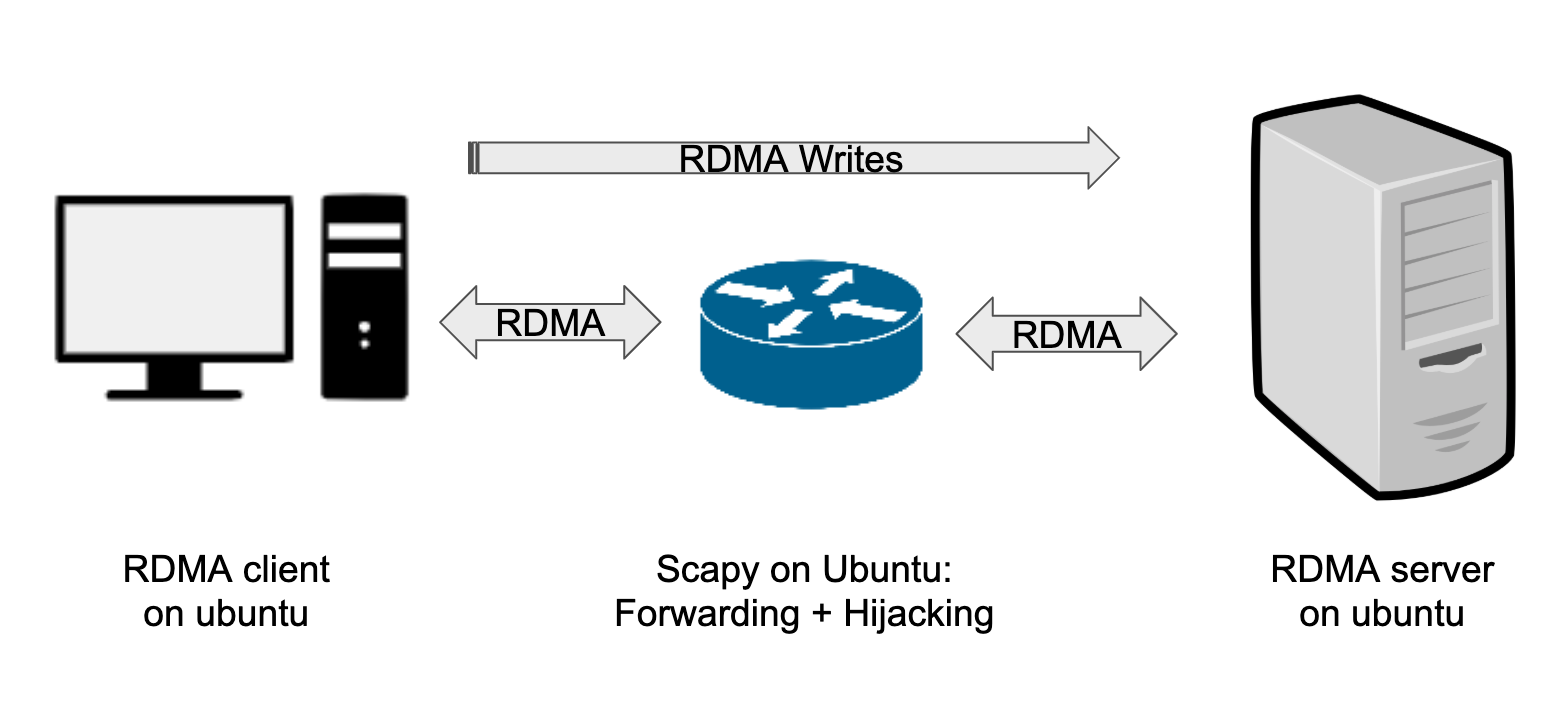
\includegraphics[width=0.5\textwidth - 5pt]{fig/attack_setup}
    \caption{Attack Testbed Setup}
    \label{fig:attack.setup}
\end{figure}

As show in \autoref{fig:attack.setup}, we run regular RDMA client and server
on two Ubuntu servers. Both machines are connected to the machine in the middle,
which uses \texttt{scapy} to sniff all \texttt{RoCEv2} packets, re-write the MAC
addresses and forward it to the other port. In the case of attackers present, we
allow the attacker to modify the packet as needed, after which we'll re-compute
the \texttt{RoCEv2} checksum according to the IBTA specs \cite{infiniband:iba.spec.vol1.v1.3},
RoCE annex \cite{infiniband:iba.spec.annex.roce} and RoCEv2 annex \cite{infiniband:iba.spec.annex.rocev2}.

We set up the \texttt{arp} entries manually such that both client and server think
they are talking to the each other directly, but in reality, the packets will all
go through the middle machine.

\texttt{scapy} is a \texttt{Python} module that allows packet sniffing, manipulation, injection, etc.
It internally calls \texttt{tcpdump} and works on raw socket as well, which gives us the ability to
re-write Ethernet-layer MAC addresses.

\subsection{Attack Model}
\label{sec:attack.model}

For the proof-of-concept attack, we choose to hijack the write address of RDMA write requests.

\begin{figure}[h]
    \centering
    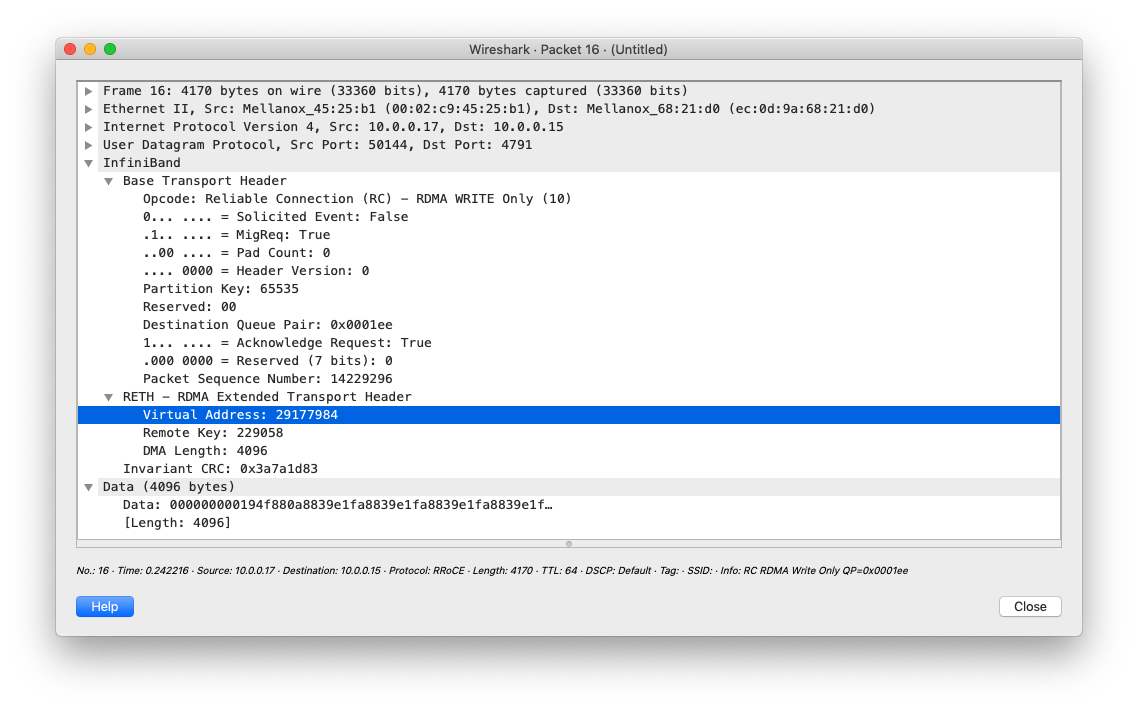
\includegraphics[width=0.5\textwidth - 5pt]{fig/rdma_write_packet_wireshark}
    \caption{RDMA Write Packet in Wireshark}
    \label{fig:attack.rdma_write_packet}
\end{figure}

RDMA WRITE allows the requestor/client to write data to the address space of the target application
on the target machine / server, using a remote key negotiated via prior authentication. However,
neither the key nor the virtual address is encrypted, as show in \autoref{fig:attack.rdma_write_packet}.

We decided to hijack all writes to the same address, which can be handy to carry out Throwhammer attack
as previously shown \cite{216055}.
For our PoC, our adversary remembers the virtual address of the first WRITE it sees,
and changes addresses of all subsequent WRITEs to be the same.

\subsection{RDMA Client/Server}
\label{sec:attack.rdma_app}

For simplicity, our RDMA client will issue $n$ RDMA WRITE requests after initial handshake and
information exchange needed for one-sided RDMA operations like RDMA WRITE. According to the attack model
described in \autoref{sec:attack.model}, our attacker hijacks all subsequent RDMA WRITEs. Thus, we compare:
1) client issues on RDMA write, and 2) client issues two RDMA writes to two different address.

We used a modified RDMA performance benchmark tool, which in the first case, issues one RDMA WRITE of 16 bytes,
and the second case, issues two consecutive RDMA WRITEs of 16 bytes each. At the end, both client and server
computes the SHA1 checksum of the buffer region. If the SHA1 digest matches, then it means all data have been
transferred successfully and not been tampered with.

\begin{table*}[ht]
    \begin{tabular}{c|c|c}
        Experiment \# & $1$ & $2$ \\ \hline
        SHA1 digest (client) & 609f05f73fb251aec1c7d8b25b4cbe1d2d1a1661 & b262a891b5dfc43930d6aa733e9741e625126a89 \\
        SHA1 digest (client) & 609f05f73fb251aec1c7d8b25b4cbe1d2d1a1661 & 2488224f4d0dff339e01d1694a0bee162eb8c358 \\
    \end{tabular}
    \caption{RDMA Proof-of-Concept Result}
    \label{table:attack.result}
\end{table*}

\subsection{Result}
\label{sec:attack.result}

As show in \autoref{table:attack.result}, in the first case, there is only one RDMA WRITE, so the attacker doesn't
modify the requests at all, thus the SHA1 digests match. But in the second case, since there are two RDMA writes, the
second RDMA WRITE is hijacked so the buffer for the second WRITE did not complete successfully. Thus the SHA1 digests
don't match. This simple proof-of-concept shows that it is (very) possible for attackers who compromised a switch to
carry out RDMA attacks like Throwhammer and more.

\section{Experimental Setup}
\label{sec:eval}

\section{Evaluation}

Here we hijack an RDMA session and learn \emph{secret} data from a the remote
memory of an unsuspecting server. Then using a similar but slightly modified
version of the attack we inject write verbs and demonstrate that we can easily
write to exposed RDMAable memory. Figure~\ref{fig:tmp} is an example of what a
figure can be.

\begin{figure}[h]
    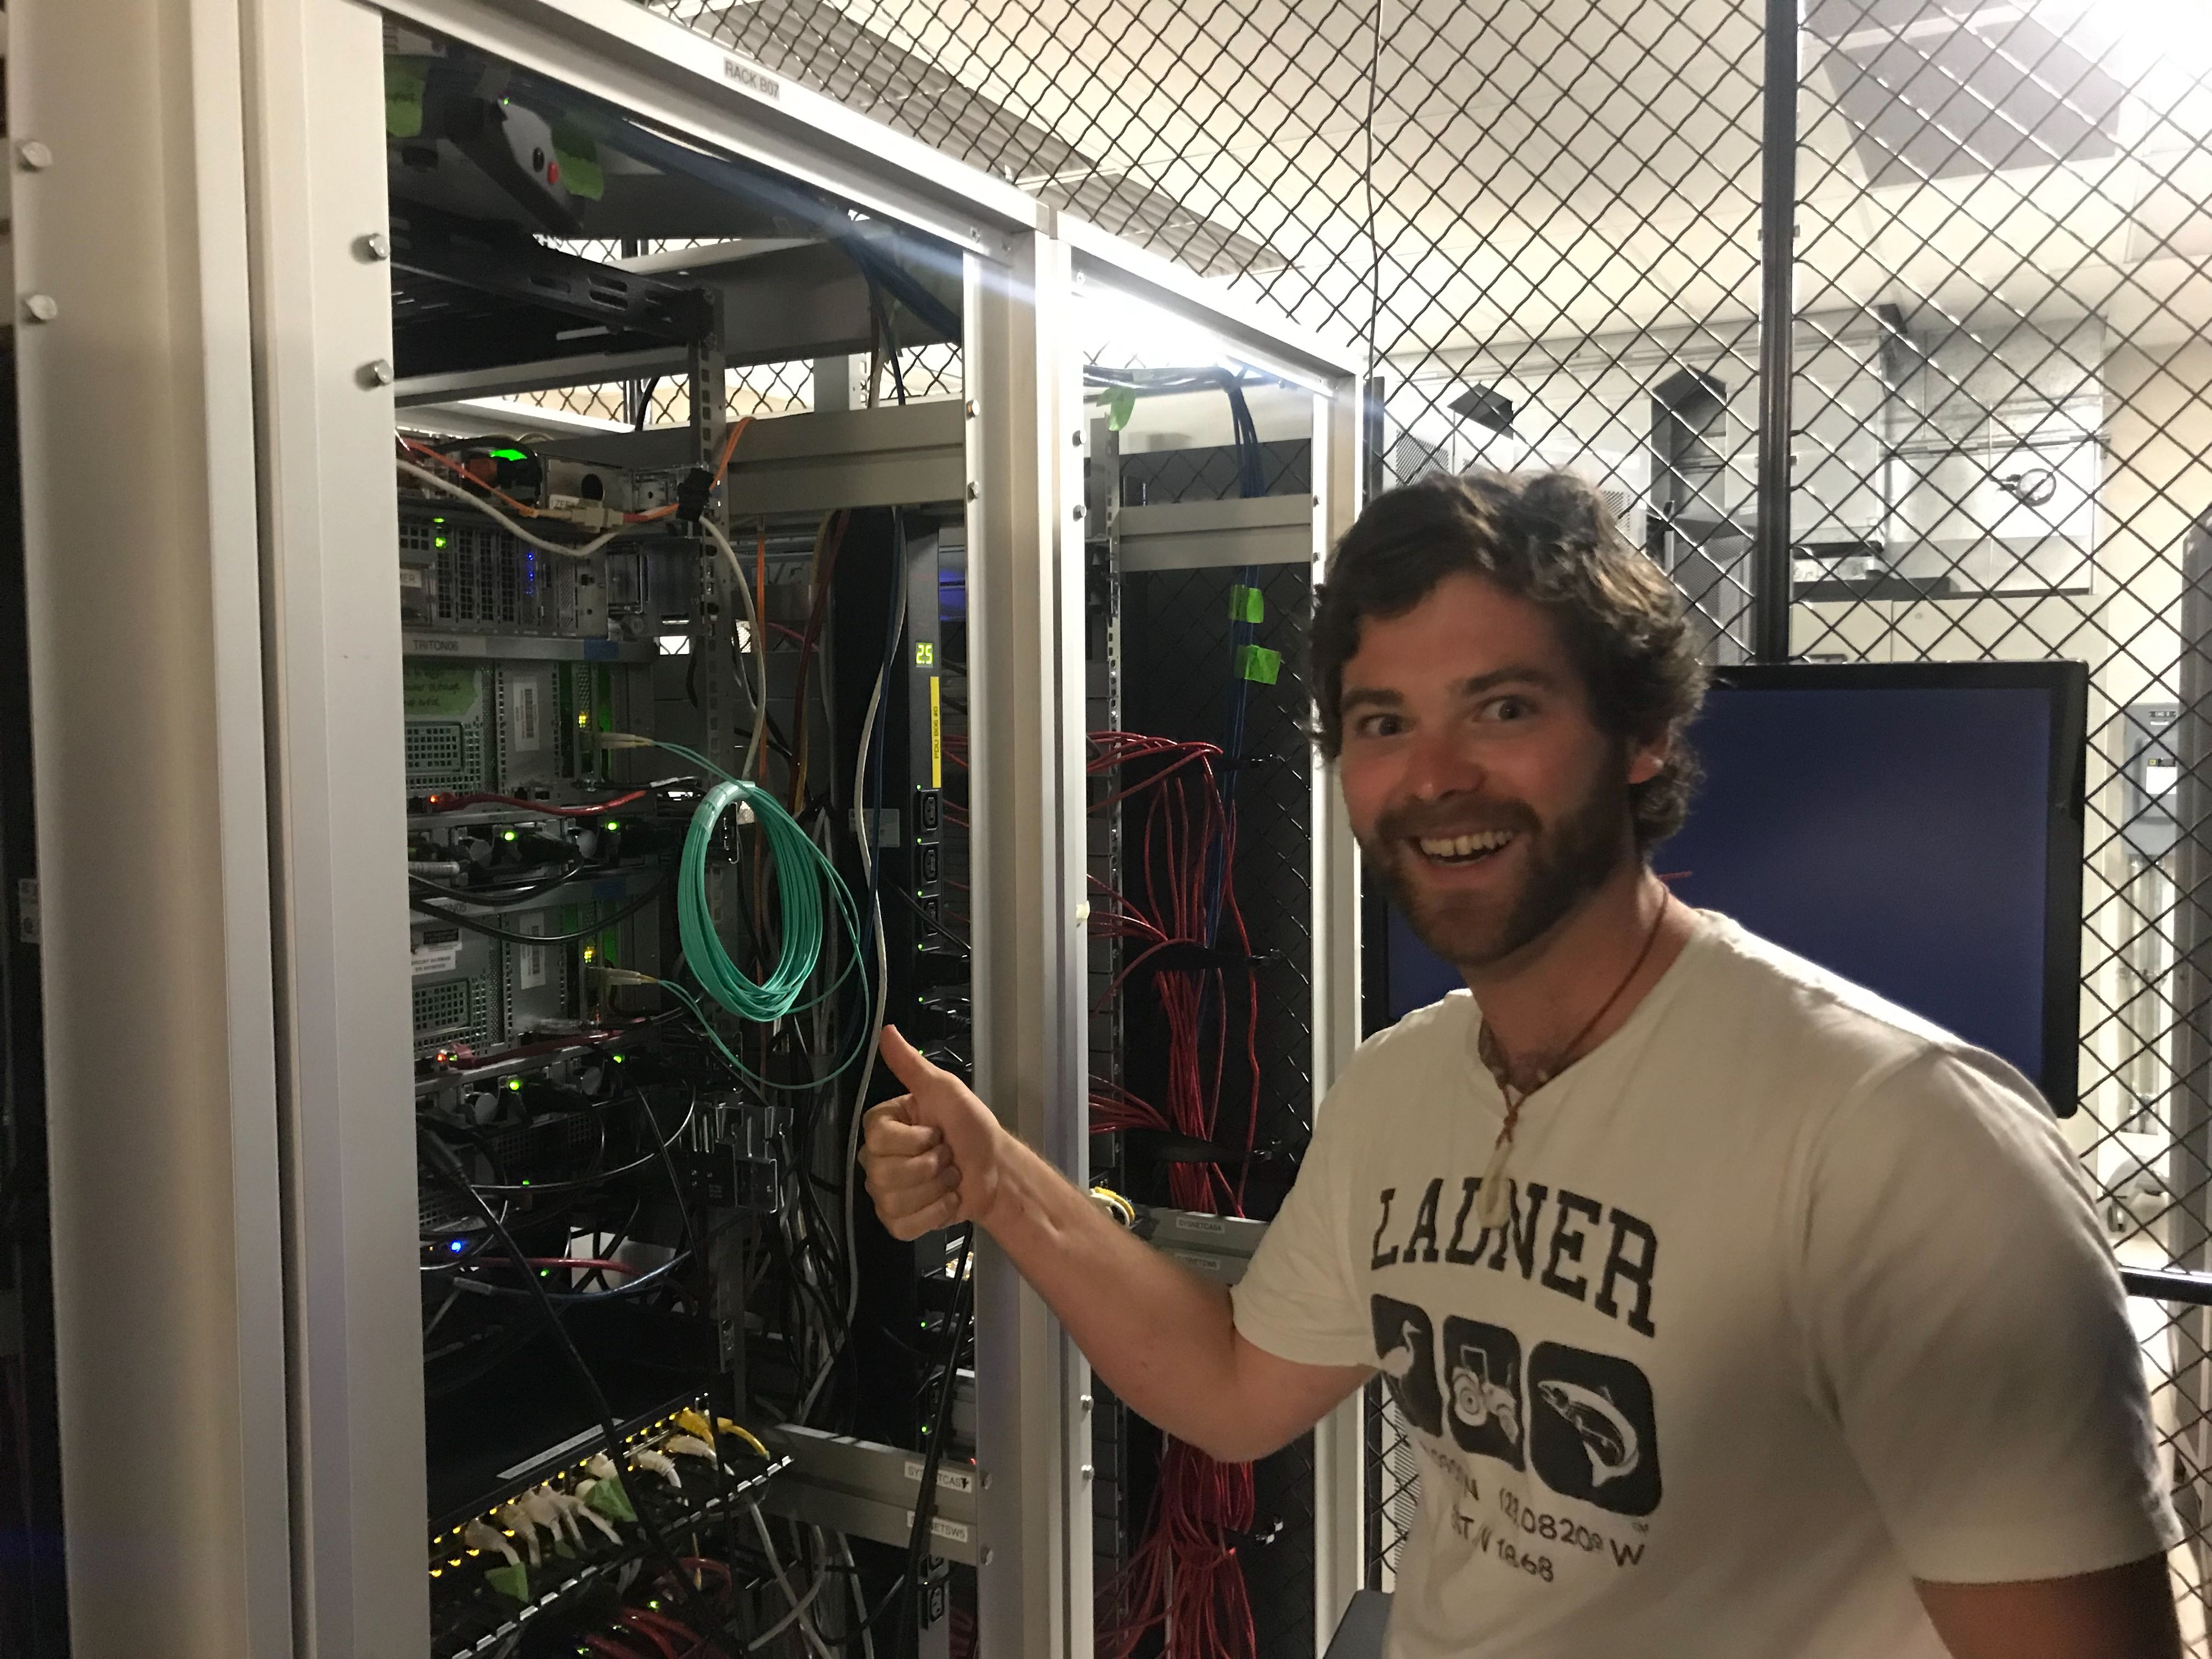
\includegraphics[width=0.5\textwidth]{fig/tmp.jpg}
    \centering
    \caption{My goodness this is a fantastic figure, it's so nice it could probably be used at a template for future figures.}
    \label{fig:tmp}
\end{figure}

\begin{table}
    \begin{tabular}{p{1.5cm}|p{1.5cm}|p{1.5cm}|p{1.5cm}}
        \hline
        \hline
    RDMA Variant & Sec prop & Verbs & Attack \\
        \hline
        RC & Seq Num & Read, Write, Send, Rec & Spoofing Seq \\
        \hline
        UC & & Read, Send, Rec & Read  \\
        \hline
        UD & Queue Pain Key & Send, Rec & \\
        \hline
    \end{tabular}
    \caption{A table roughly describing RDMA security primitives}
    \label{table:attacks}
\end{table}


\section{Conclusion}
\label{sec:conclusion}

All of our work should be encorporated into RoCEv3





\balance
\vspace{-0.3cm}
{\footnotesize \bibliographystyle{acm}
\bibliography{paper}}
\vspace{-0.5cm}

\end{document}
